%\documentclass{article}
%\usepackage{graphicx,subfigure}
%\begin{document}

\begin{figure}[!h]
  \centering
   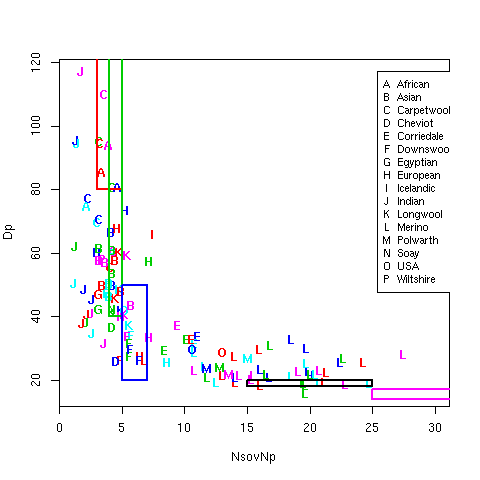
\includegraphics[width=1.0\textwidth]{NsovNpDpa.png}
  \caption{Plot of breed means of $N_{s}/N_{p}$ and $D_{p}$ for 126 flocks sampled by Carter(1968)~\cite{cart:68}. The breeds have been grouped into a {\em breed type} which in some cases is an individual breed and in other cases is a country of origin. The coloured rectangles represent the approximate ranges of measurements for sheep representing Ryder's 4 stages of Merino Evolution, plus the Modern SRS Fine Merino. Red rectangle is Wild stage, green is Hairy Medium Wool, blue is Generalised Medium Wool, black is Finewool Merino, and magenta is SRS Fine Merino.}
  \label{fig:NsovNpDpa}
\end{figure}

%\end{document}

